\begin{frame}
  \frametitle{What is goal-oriented error control? \\
    {\small The scientist's viewpoint}}
  \begin{center}
    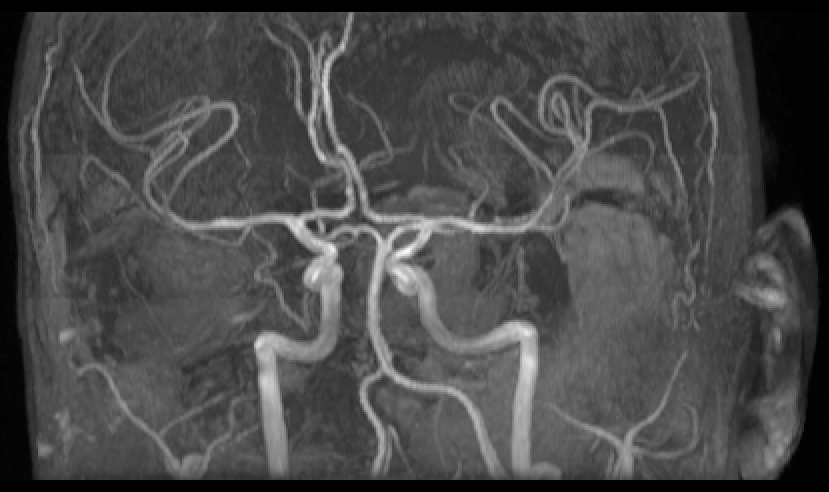
\includegraphics[height=3.5cm]{png/circle_of_willis_scan.png} \hspace{0.3cm}
    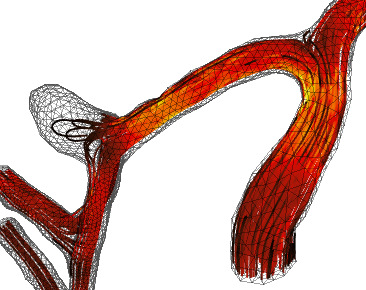
\includegraphics[height=3.5cm]{png/circle_of_willis_aneurysm.png}
    \\
    \vspace{3.0em}
    Shear stress at vessel wall?
  \end{center}
%    {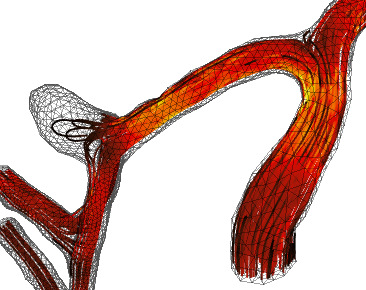
\includegraphics[width=0.4\textwidth]{png/circle_of_willis_aneurysm.png}};
%  \begin{tikzpicture}
%    \node at (0,1)
%    {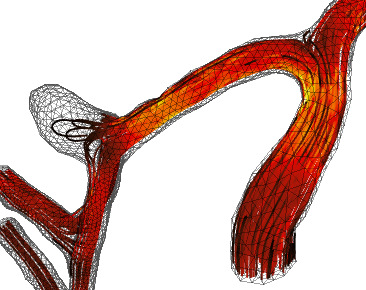
\includegraphics[width=0.4\textwidth]{png/circle_of_willis_aneurysm.png}};
%    \node at (5,-1){\includegraphics[width=0.6\textwidth]{/home/meg/presentations/slides/eps/vessel.png}};
%    \node at (5, 2){Quantity of interest:};
%    \node at (5, 1.5){Shear stress at vessel wall?};
%  \end{tikzpicture}
\btVFill
{\tiny [Valen-Sendstad '08]}
\end{frame}
